
% This LaTeX was auto-generated from MATLAB code.
% To make changes, update the MATLAB code and republish this document.

\documentclass{article}
\usepackage{graphicx}
\usepackage{color}

\sloppy
\definecolor{lightgray}{gray}{0.5}
\setlength{\parindent}{0pt}

\begin{document}

    
    \begin{verbatim}
clear;clc

A = [0 0;2 0];
B = [2;0];
C = [0 1];
eig(A)
cm =ctrb(A,B);
rank(cm)
om = obsv(A,C);
rank(om)

K = [0.707 0.250];
L = [100;50];


% initialization
x(:,1) = [5;-4];
y(:,1) = C*x(:,1);
x_hat(:,1) = [0;0];
y_hat(:,1) = C*x_hat(:,1);
t = 0:0.01:20; %0.01 time span of interest
nt = length(t); % number of time steps
dt = t(2) - t(1);
kg = 1;

% reference input
for i = 1:nt
    r(:,i) = sin(i*dt);
end

% case 2: state-feedback
u(:,1) = -K*x(:,1) + kg*r(:,1);
for i = 1:nt-1
x_dot(:,i) = A*x(:,i) + B*u(:,i);
x_hat_dot(:,i) = A*x_hat(:,i) + B*u(:,i) - L*(C*x_hat(:,i)-y(:,i));
x(:,i+1) = x(:,i) + x_dot(:,i)*dt;
x_hat(:,i+1) = x_hat(:,i) + x_hat_dot(:,i)*dt;
y(:,i+1) = C*x(:,i+1);
y_hat(:,i+1) = C*x_hat(:,i+1);
u(:,i+1) = -K*x(:,i+1) + kg*r(:,i+1);
end
figure
plot(t,r(1,1:nt),'k--',t,x(1,:),'b',t,x_hat(1,:),'r','linewidth',2)
set(gca,'fontsize',18)
legend({'$r$','$x_1$','${\hat x}_1$'},'Interpreter', 'latex')
legend boxoff
xlabel('Time (s)')
figure
plot(t,r(1,1:nt),'k--',t,x(2,:),'b',t,x_hat(2,:),'r','linewidth',2)
set(gca,'fontsize',18)
legend({'$r$','$x_2$','${\hat x}_2$'},'Interpreter', 'latex')
legend boxoff
xlabel('Time (s)')
\end{verbatim}

        \color{lightgray} \begin{verbatim}
ans =

     0
     0


ans =

     2


ans =

     2

\end{verbatim} \color{black}
    
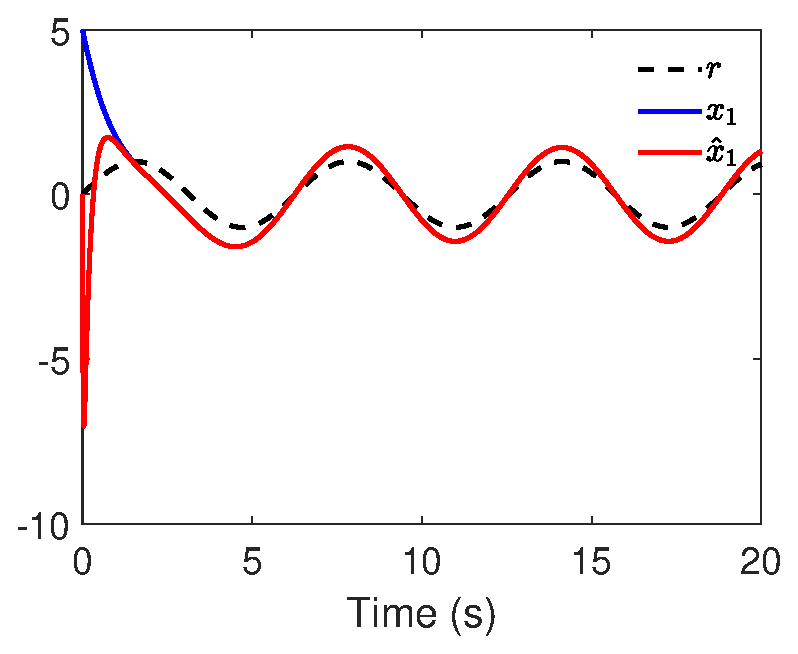
\includegraphics [width=4in]{hw8_1_01.eps}

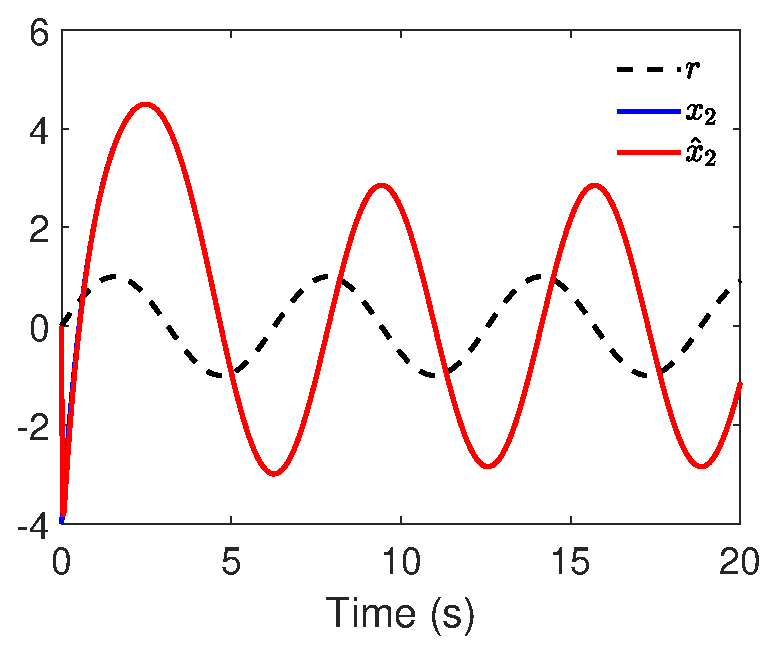
\includegraphics [width=4in]{hw8_1_02.eps}



\end{document}

